\newcommand{\novathesis}{\emph{novathesis}}
\newcommand{\novathesisclass}{\texttt{novathesis.cls}}

\chapter{Introduction}
\label{intro}

\section{Embraer S.A.}
\label{embraer}

Embraer S.A. is an airplane manufacturer which excels at Regional Jets and Private Jets. Founded in 1969, it has manufacturing and assembly sites across the world, having a big international presence. 

\subsection{Embraer Portugal S.A.}
\label{embraerpt}

In Évora, Portugal, Embraer has 2 sites: Estruturas em Compósitos S.A. (Composites manufacturing) and Estruturas em Metálicos S.A. (Metal manufacturing). 

\section{Composites: an approach}
\label{composites}

Since the beginning of mankind, history has been separated into Ages, i.e. Stone Age, Bronze Age, Iron Age, etc. We are living in an Age which cannot be described by a single material. Mankind has been using more and more resources, which have a lot of diversity and can now mix different resources and call them "composites". Make tiny little structures and call them "nanostructures". Use carbon based materials and make them the strongest materials to existence. There is not a main field of resources which can be use to describe this Age we are living in.

However, composite materials have been developed greatly the last two centuries. Even though that concrete, for example, has been used since the Egyptians Pyramids, therefore being one the one of the oldest materials used in our history. Nowadays, it is expected for composites to be the most type of material used in the world, due to the fact of its outstanding properties, achieving great strength with less weight when comparing to other kind of materials. Composites, by definition, are a mix between two main components: the matrix and the reinforcements. The matrix is the material that mantles the reinforcements and reinforcements is what is added in order to improve properties. Right now, composites have the advantage to produce what has not been able to produce with single materials matrix. 

Due to its range of properties, it is expected an incredible range of uses. Covering most of the modern day industry applications such as aeronautics, automotive, sports and construction. It ranges from the most used material in the world, concrete, to optimized carbon fiber laminates. Composites are categorized in three major groups: \textbf{M}etalic \textbf{M}atrix \textbf{C}omposites, \textbf{P}olymer \textbf{M}atrix \textbf{C}omposites and \textbf{C}eramic \textbf{M}atrix \textbf{C}omposites. Then these have 3 subcategories: Particle-reinforced, fiber-reinforced and structural (figure \ref{fig:reinforcements}).

\begin{figure}[htbp]
\setlength{\belowcaptionskip}{-15pt}
\centering
	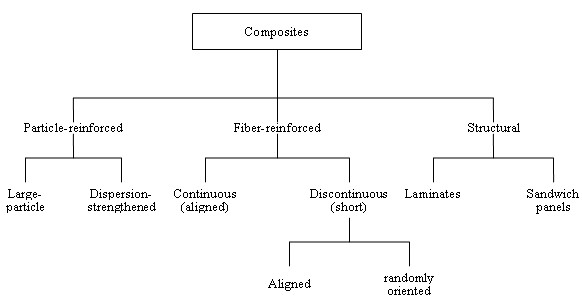
\includegraphics[scale=0.65]{reinforcements}
	\caption{Reinforcement grouping adapted from \cite{reinforcements}.}
\label{fig:reinforcements}
\end{figure}

Depending on application, each group of composite material is praised to be the solution. In aeronautics, the carbon fiber laminates are one of the most used composite materials, due to their strength to weight ratio and low thermal expansion coefficient\cite{Campbell2004}. However, along with some other composite classes, the main failure mode is the interface between the fibers and the matrix. This is a major concern since this deficiency is highly damaging for the material if measures are not applied. As such, there is a great need to evaluate and measure the composite interface failures with mechanical tests as these will provide the most genuine failure compared to the real world. These tests will be described in section \ref{sub:mechanical} and chapter \ref{mechanical}. Most concepts and terminology used in aeronautics and this particular thesis are defined at ASTM D3878 \cite{D3878}.

\subsection{Carbon Fiber Reinforced Polymers}
\label{prepregs}

\gls{cfrp} demand research to find out the right material mixture since the ratio between resin and fiber is highly regarded in the final properties of the laminate. In addition, the process used is a big factor as well. Impregnating the resin whilst doing hand lay-up is not really the best solution. It will not create homogeneity and provoke resin accumulations. This will put the physical integrity of the resin/carbon fiber bond. Because of this, suppliers arranged a new set of material, preimpregnated carbon fiber, or simply, prepregs. This material comes with the carbon fiber embed with resin, so that the client does not need to worry about the mixing of this two products. The mix is already made to guarantee perfect fiber/epoxy matrix and ensures little to no variation. Prepregs come in various shapes and forms, but there are three main groups of carbon fiber prepregs: tape, tows or fabric. These products usually come in B stage (detailed at \ref{cure}), one of the curing stages, to ensure better handling \cite{Aviation}

Thermoset and thermoplastic matrix are used in prepregs, although it is far more common to use thermoset resin, for example epoxy, polyester and vinyl ester. The main disadvantage of using a thermoset matrix is that it cannot be reprocessed. In the specific case of thermoset resins, after curing, the material cannot undergo another molding process. Since the mixture of resin, cure process starts to develop from room temperature. Slowing down the cure process is achieved by reducing the temperature (more information on section \ref{cure}). This room temperature condition restricts the amount of hours the material has on room temperature, in terms of molding and layup processing, until it reaches a state of no processability. This defines and highlights the definition of out time and shelf life. It becomes a necessity to control out time to assure perfect material processability\cite{Morgan2005}.

Carbon fiber range of applications vary depending on which precursor polymer is used, with many precursors being studied to produce carbon fiber while easy conversion to carbon fiber, high carbon yield and cost-effective processing being the main searched characteristics of the precursors used\cite{Campbell2004}. The most popular precursors used are:

\vspace{-\topsep}
\begin{enumerate}
	\setlength{\parskip}{0pt}
	\setlength{\itemsep}{0pt plus 1pt}
	\item \textbf{Acrylic precursors} - Which have been the most successful in the industry world, with PAN being the most popular acrylic precursors for quite some time now;
	\item \textbf{Cellulosic precursors} - While containing around 44\% carbon, the process is more than simple dehydration, like Edison's filaments, and the carbon yield is only  around 25\%.
	\item \textbf{Pitch-based precursors} - In spite of having a 85\% carbon yield, these precursors give carbon fiber a high modulus, due to the graphical nature of these fibers, although the fibers have poorer compression and transverse properties compare to Acrylic precursors.
\end{enumerate}
\vspace{-\topsep}

Other precursors, like Vinylidene chloride and phenolic resins are used as well, but were found not commercially viable.

\subsubsection{Resin}
\label{resin}

Thermoset resins, unlike thermoplastic resins, are defined by having a cure reaction. Thermosets are used over thermoplastics as result of its wide range of properties without changing any structure, by altering the amount of crosslinks in thermoset network. Since 90\% of thermoset resins used are polyester resins, as consequence of being cheap to make, it would be expected for them to be used as matrix in prepregs. However, the resins with better mechanical and high temperature performance are used. Epoxy resins are the next most important class of resins and there are no alike in all thermoset resin classes\cite{Ratna}. This is justified by several reasons:

\vspace{-\topsep}
\begin{enumerate}
	\setlength{\parskip}{0pt}
	\setlength{\itemsep}{0pt plus 1pt}
	\item Low volume reduction after cure, therefore less residual stress inducted by resin shrinkage in laminate, than most thermosets;
	\item Possibility of a wide range of temperature, by choosing thoughtfully the curing agents to enable a good degree of crosslinking control;
	\item Less applied pressure needed for fabrication of products, compared to other thermoset resins;
	\item Possibility of having a range from low viscous liquid to tack-free solid.
\end{enumerate}
\vspace{-\topsep}

Because of this, epoxy resins are used in a wide variety of applications, including adhesives, coatings, composites, but when needed, higher functionality epoxy are used in aerospace and critical defense applications \cite{Ratna}. Regarding versatility, epoxy resins can cure using an array of materials, with various types of curing conditions. Epoxy resin is chemically described as a low molecular weight organic liquid containing a group of epoxide groups, illustrated in figure \ref{fig:epoxygroup}, which are three member rings of two carbon atoms and an oxygen atom. Cure reactions and more details at section \ref{cure}.

\begin{figure}[htbp]
\setlength{\belowcaptionskip}{-15pt}
\centering
	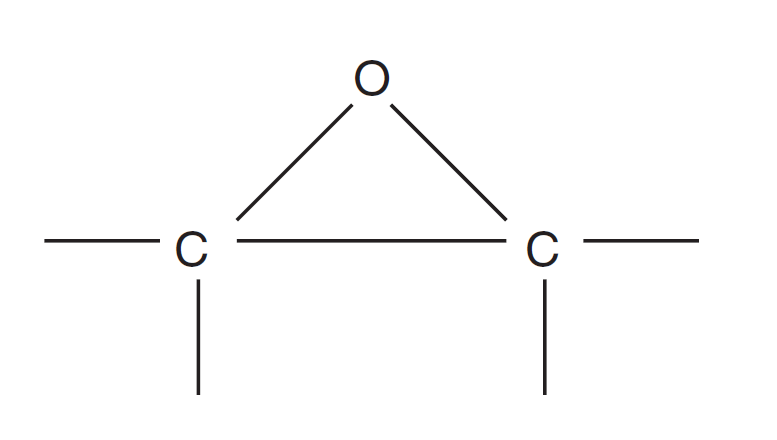
\includegraphics[scale=0.25]{epoxygroup}
	\caption{Illustration of a three member ring epoxy group. \cite{Ratna}}
\label{fig:epoxygroup}
\end{figure}

\subsection{Composite Laminates}
\label{laminates}

In this thesis subject, laminates are continuos carbon fiber reinforced epoxy resin which are laminated through hand layup or automated layup (more details on \ref{layup}). The carbon fiber continuos reinforcement will provide strength in the orientation of said fibers. However, in the perpendicular direction, 90º, load is absorbed by the matrix, therefore, strength is characterized by the matrix, which is notoriously weaker. Therefore, it is logical to design a laminate containing fibers oriented in multiple directions. Campbell \cite{Campbell2004} defines a quasi-isotropic laminate as a balanced laminate with equal number of plies in the 0º, +45º, -45º and 90º. This proposal is highly regarded as optimal, since it provides laminates with great strength in multiple orientations.

\begin{figure}[!htbp]
\setlength{\belowcaptionskip}{-10pt}
\centering
	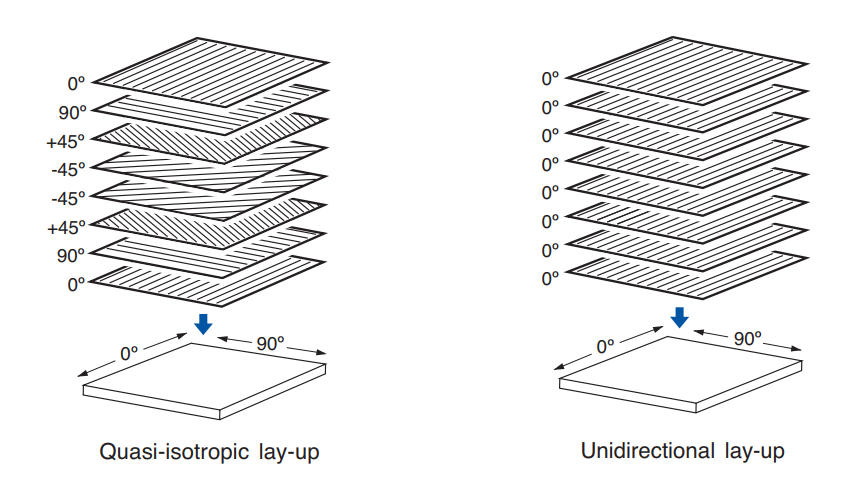
\includegraphics[scale=0.45]{layup}
	\caption{Orientations in a laminate and an example of a quasi-isotropic laminate adapted from \cite{Hexcel}}
\label{fig:epoxygroup}
\end{figure}

Mechanical properties can be considered as a specific job appointed either to the matrix or the reinforcement. Longitudinal strength and compression loads are appointed to fibers whereas the matrix disperse the load between the fibers and prevents the fibers from deforming under compression. A summary is provided in table \ref{table:properties}. \cite{Campbell2004}

\begin{table}[!htbp]
\centering
\setlength\aboverulesep{0pt}\setlength\belowrulesep{0pt}
\caption{Summary of dominating composite constituent on each mechanical properties, adapted from \cite{Campbell2004}.}
\label{table:properties}
\begin{tabular}{@{}r|c|c@{}}
                                                                                                     & Mechanical Property & Dominating Composite Constituent \\ \midrule
\parbox[t]{2mm}{\multirow{4}{*}{\rotatebox[origin=c]{90}{{\scriptsize \textbf{Unidirectional}}}}}    & {\footnotesize 0º Tension}          & {\footnotesize Fiber}                            \\
                                                                                                     & {\footnotesize 0º Compression}      & {\footnotesize Fiber}                            \\
                                                                                                     & {\footnotesize Shear}               & {\footnotesize Fiber and Matrix}                 \\
                                                                                                     & {\footnotesize 90º Tension}         & {\footnotesize Matrix}                           \\ \midrule
\parbox[t]{2mm}{\multirow{4}{*}{\rotatebox[origin=c]{90}{{\scriptsize \textbf{Laminate}}}}}          & {\footnotesize Tension}             & {\footnotesize Fiber}                            \\
                                                                                                     & {\footnotesize Compression}         & {\footnotesize Fiber and Matrix}                \\
                                                                                                     & {\footnotesize In-Plane Shear}      & {\footnotesize Fiber}                            \\
                                                                                                     & {\footnotesize Interlaminar Shear}  & {\footnotesize Matrix}                          
\end{tabular}
\end{table}


\section{Fabrication}
\label{fabrication}

Fabrication is where parts are manufactured. It follows a workflow designed to be fast and accessible. That flow follows the same organization as the following sections:

\vspace{-\topsep}
\begin{itemize}
	\setlength{\parskip}{0pt}
	\setlength{\itemsep}{0pt plus 1pt}
	\item Freezer and Cutting room
	\item Layup process
	\item Cure process
	\item Quality assurance
\end{itemize}
\vspace{-\topsep}

Each workstation has a specific purpose and serves as a main facilitator to achieve product quality. As factory layout follows lean strategy, paths and movement are optimized, reduced and close to each workstation. 

\subsection{Freezer}
\label{freezer}

When a material is received, it has to be stored in a special environment to minimize the cure process at room temperature. Suppliers tend to suggest a temperature to store the material, usually around -18ºC. This allows the storage and usage of the material when necessary, without worrying about the integrity of the material. The lean strategy used is First In First Out, where the oldest batch is the first at being used in production, while preserving the newest batch.

Using a specific stock management software, material out time is controlled, as well the quantity of material used in each production. Control over exposure temperature is highly recommended by suppliers to ensure B stage is maintained and to keep room temperature curing from occurring.

\subsection{Layup Process}
\label{layup}

As one of the most used process in composites world, layup process consists in the stack of plies in a specific sequence and orientation where either hand layup or automated layup processes can be used. Laminates produced by such method can be oriented to enhance the strength of the material in a primary load direction. Therefore, as such, laminate orientation and thickness are highly crucial, having a direct influence on its mechanical properties. Although thickness is directly correlated with major mechanical properties improvement, orientation provides a quasi-isotropic layup, as mentioned above in \ref{laminates}. 

As most manufacturing processes, layup processing has both advantages and disadvantages. Advantages are easy manufacturing, no big thermal, mechanical or chemical reactions involved, except for the resin cure. It has as disadvantages regarding the complexity of the part, as sole process, and investment value.

There are many factors that have to be considered while laying up, such as angling, defects (porosity, wrinkles, material excess or lack of material, etc.) and gaps. Porosity and wrinkles are consequence of lack of applied pressure during layup.  Gaps are supposed to follow under rules, e.g. staggering, in order to have something that fulfills the gap in the next ply and improve part cohesiveness.

\subsubsection{Hand Layup}
\label{hlayup}

Hand Layup is the process of manual layup and it's done mostly due to more small, intrinsic or complex geometries, where automated layup isn't just able to perform. Highly qualified employees layup ply after ply with help of laser guidance and specialized tools. 

The major drawbacks on this process is high labour costs, low production rates and variability (from laminator to another) \cite{Skramstad}.

\subsubsection{Automatic Layup - Automated Tape Layup}
\label{atlayup}

\gls{atl} is an automated layup machine which uses tape of carbon fiber prepregs, described in \ref{prepregs}. A single tape of 150mm wide is usually used, although other sizes (300mm or 75mm) and combinations (single tape, double tape or multitape (four tapes) combination). Most manufacturers store layup material right above the roller head as ilustrated in \ref{fig:atlheadschem}. ATL machinery had a development burst in 1980s, in terms of layup speed and 1990s, in terms of layup quality. \cite{Lukas}

This machine works using CNC programming, as well as \gls{afp} and Embraer's Waterjet cutting machine. As intended, gaps are induced and controlled within a range to reduce lost mechanical performance. 
Machine with 5 axes of freedom, has a head like one illustrated in \ref{fig:atlheadschem}, where material is heated prior to layup, applying force through a roller to consolidate ply operation. Even as the one of the oldest automated layup processes \cite{Lukas}, \gls{atl} is a very useful resource in aeronautic industry. However, \gls{afp} came as an improvement to ATL, allowing for more complicated geometries and fewer waste compared to ATL process.

\begin{figure}[htbp]
\setlength{\belowcaptionskip}{-10pt}
\centering
	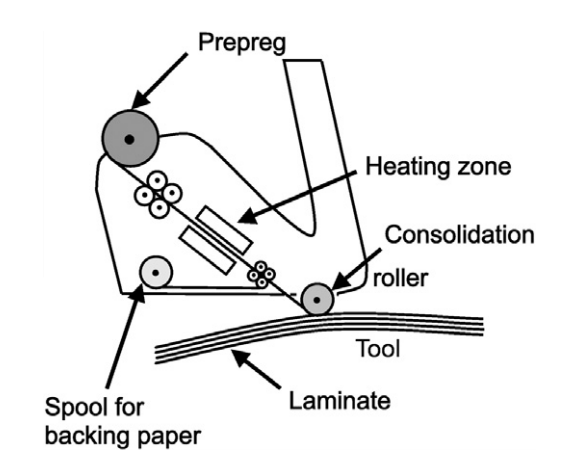
\includegraphics[scale=0.6]{atlheadschem}
	\caption{Design of a common ATL head adapted from \cite{Astrom}.}
\label{fig:atlheadschem}
\end{figure}

\subsubsection{Automatic Layup - Automated Fiber Placement}
\label{afplayup}

\gls{afp} machine was introduced in 1974 by Goldsworthy, being an ATL machine head with a slitting unit which slit tape into individual tows \cite{Goldsworthy}. Commercially introduced in 1980s, developed in the early 2000's, it's a machine with a  with 6 axes of freedom, cooling material and warms where material is going to be laminated. The \gls{afp} machine head is exemplified at \ref{fig:afpheadschem}, where some differences can be noted to the ATL machine head.

\begin{figure}[htbp]
\setlength{\belowcaptionskip}{-15pt}
\centering
	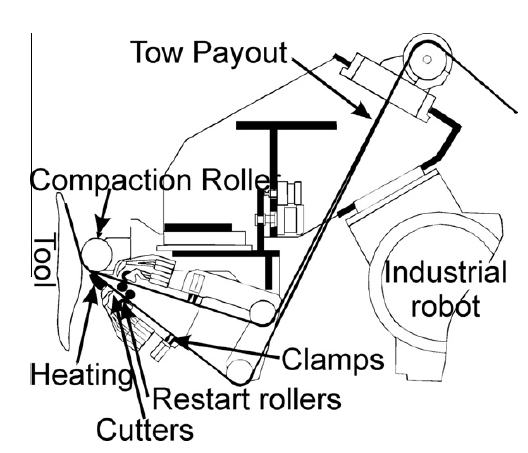
\includegraphics[scale=0.6]{afphead}
	\caption{Design of a common AFP head adapted from \cite{Lukas}.}
\label{fig:afpheadschem}
\end{figure}

One of the differences in AFP to ATL processing is the material width. Whereas 150mm tape is the most common in ATL machine systems, 6,4 mm tow is the most common in AFP machine systems. The amount of tows is what characterizes the width of AFP lamination process, where some systems go up to 32 tows in a single sequence. Each tow is treated as one individual tow, allowing to cut, add and clamp one tow individually, allowing tow steering, for example. Tow width and number of tows depends highly on local geometry and complexity, providing us with the ability to adapt to these situations. AFP process productivity is lower than ATL rate since AFP normally is used to manufacture complex parts.

\subsection{Hot forming process}
\label{hd}

Hot forming is a mechanical process which forms the material to a mold using both temperature and pressure as auxiliary forces. While temperature is achieved with heating lamps, pressure is achieved with vacuum pumps. The hot forming cycle has 6 steps:

\vspace{-\topsep}
\begin{enumerate}
	\setlength{\parskip}{0pt}
	\setlength{\itemsep}{0pt plus 1pt}
	\item Heating ramp;
	\item Temperature stabilizing;
	\item Vacuum starting ramp;
	\item Hot forming baseline - Maximum temperature and pressure;
	\item End of vacuum;
	\item Cooling ramp;
\end{enumerate}
\vspace{-\topsep}

While having a cycle similar to curing cycle, the temperature and pressure are lower. While temperature is assigned to be within room temperature and cure reaction temperature, pressure is near the pressure used in Autoclave during cure cycle. The heating ramp, laminate thickness, system pre-heat and cooling ramp are definite factors to temperature uniformity. While this process is highly useful, due to the capacity to manufacture tight angles without porosity, the heat cycle deals a great tool to the prepreg resin. This reduces prepreg properties and may damage the prepreg to the point of no return. Being the main objective of this thesis, this work will look into the damage into prepreg resin and analyze it to assess its effects on aging material.

\subsection{Cure}
\label{cure}

The epoxy resin cure is defined in three different stages \cite{Aviation}:

\vspace{-\topsep}
\begin{itemize}
	\setlength{\parskip}{0pt}
	\setlength{\itemsep}{0pt plus 1pt}
	\item A-stage: When both epoxy components, the base and the curing agent or hardener, are mixed but without any chemical reaction.
	\item B-stage: Intermediate state when chemical reaction has already started and material gets thickened and tacky. This stage is maintained when stored at -18ºC.
	\item C-stage: Fully cured resin.
\end{itemize}
\vspace{-\topsep}

%cura no autoclave é pressão atmosférica, hot forming é pressão de vácuo.

These stages are set to easily understand cure reaction and define curing phases in order to easily evaluate the curing degree of a material. As said before, cure reaction starts when both curing agent and base material are mixed. These curing agents, or hardeners, are picked regarding the applicable curing conditions and resin final application. The curing reaction is initiated with a reactive curing agent reacting with two epoxy rings where two different reactions occur in this specific case an amine curing agent. First there's a reaction between the primary amine group hydrogen and the carbon in the epoxy group. Then, the secondary amine group hydrogen bonds with carbon in epoxy group. This reaction is exemplified in figure \ref{fig:epoxycure}. 

\begin{figure}[htbp]
\setlength{\belowcaptionskip}{-10pt}
\centering
	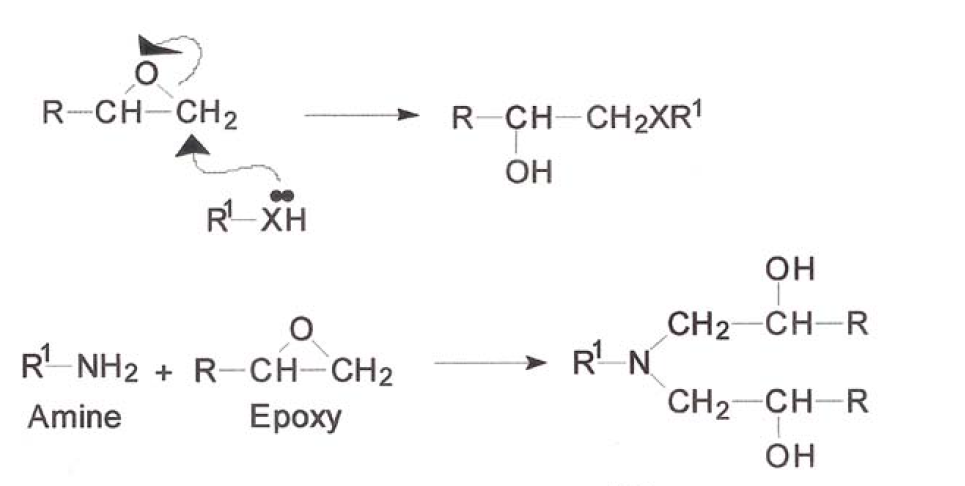
\includegraphics[scale=0.3]{epoxycure}
	\caption{General cure process for epoxy resins using amine curing agent. \cite{Ratna}}
\label{fig:epoxycure}
\end{figure}

The kinetics of this reaction are lead by temperature and time. To assess the relation between rate and degree of cure a lot of kinetic models have been developed over the years. Global reaction kinetic reactions are most used to characterize thermoset polymers (i.e. epoxy resin). Kinetic parameters of cure reaction can be found through DSC analysis. Adapting and citing Hardy \cite{Ricky}, data gathered from DSC equipment can be fitted into kinetic reaction models. Assuming that the rate of heating is proportional to rate of reaction, as written below:

\begin{equation}
\label{eq:dsckineticreaction}
\gls{degreecure} = \dfrac{\gls{heatreaction}}{\gls{heatreactiontotal}}
\end{equation}

Assumption is made that the equation can be split and defined by two separate equations, $K(T)$ and $f(a)$, which help us define reaction cure accordingly:

\begin{equation}
\label{eq:assumption}
\gls{degreecure} = \gls{tdrc}\times\gls{reactionmodel}
\end{equation}

However, heat dependence of the reaction rate is commonly defined as an Arrhenius equation, which is characterized as follows:

\begin{equation}
\label{eq:arrhenius}
\gls{tdrc} = A \exp \left (\dfrac{-\gls{activationenergy}}{\gls{gascte} T}  \right )
\end{equation}

When combined and defining heating rate as $\beta = \dfrac{dT}{dt}$, the cure reaction can finally be defined as:

\begin{equation}
\label{eq:cure}
\gls{degreecure} = \dfrac{A}{\beta} \exp \left (\dfrac{-\gls{activationenergy}}{\gls{gascte} T}  \right ) \gls{reactionmodel}
\end{equation}

There have been multiple kinetic reaction models which fit cure reaction, however, $n^{th}$ order model, expressed in equation \ref{eq:nthorder}, usually depicts thermoset cure behavior. Assuming a kinetic model and using equations above, cure reaction and its parameters can be predicted in a given temperature or heating rate.

Using $n^{th}$ order model, the final equation is presented as such:

\begin{equation}
\label{eq:nthorder}
\gls{degreecure} = \dfrac{A}{\beta} \exp \left (\dfrac{-\gls{activationenergy}}{\gls{gascte} T}  \right ) (1-\alpha)^n
\end{equation}

Thus endorsing the key element that the degree of cure is directly correlated to temperature and time. However, for an homogeneous cure, activation energy must be provided to the resin for proper cure reaction and flow of resin. It is also important for proper cross-linking.

\subsubsection{Autoclave cure and vacuum bagging}
\label{chap:vacuumbag}

As depicted, it is necessary to cure \glspl{cfrp} to end up with a finished and solid product. This process is usually done with the aid of a equipment called autoclave. Autoclave is, according to Kuppers J. and Walczyk, D. <inserir referência>, a large pressure vessel that allows the simultaneous application of heat, vaccum within the bagged part and external pressure to the laminate. While being inefficient, it is the option that guarantees best quality product. This process requires the laminates to be within a vacuum bag to ensure part consolidation, obtained by vacuum system in autoclave which removes most volatile substances. This reduces porosity in the product. Vacuum bag also aids in pressurizing the product to assure a good, even product.

Autoclave process cycle combining temperature, pressure and vacuum is exemplified in figure \ref{fig:autoclave}. 

\begin{figure}[htbp]
\setlength{\belowcaptionskip}{-10pt}
\centering
	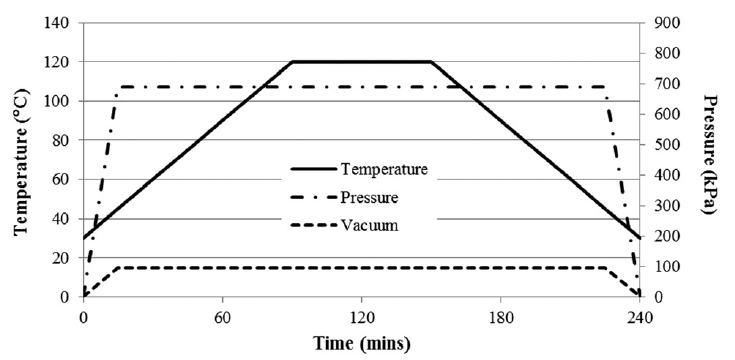
\includegraphics[scale=0.3]{autoclave}
	\caption{Example of an Autoclave process cycle, adapted from <inserir a referência>}
\label{fig:autoclave}
\end{figure}


\subsection{CNC waterjet cutting and finishing}
\label{chap:waterjet}

CFRP cutting is a very meticulous operation, due to the necessity of finishing with a clean cut and how hard it can be to cut carbon. With metallic blades, cut can be extremely hard since the cut would make the blade hot and that would damage the CFRP laminate through delamination where the blade would cut. Even with proper lubrication, the cut would be defined with scratches and probable delamination. This also ruins the blade and those designed to cut cured CFRP laminates are expensive. This result in a poor 

\subsection{Quality Assurance}
\label{chap:ultrasons}

